\section*{Dataset}
	 We are using Cancer dataset, which are published as MedQuAD dataset~\cite{DBLP:journals/corr/abs-1901-08079}. This dataset is specifically created for medical question-answering. The dataset created from 12 NIH websites (e.g. cancer.gov, niddk.nih.gov, GARD, MedlinePlus Health Topics). The Cancer dataset are focused on 98 types of cancers, and each type of cancer can have maximum 12 types of questions. In total we have 729 questions, and their questions types are distributed as Table~\ref{tab:count-qtypes} and Figure~\ref{fig:cancer-type-qtype-count}:
 	\begin{table}[b]
	\caption{List of the question type and their count}
	\label{tab:count-qtypes}
 		\begin{tabular}{ll}
 			\toprule
 			Question type&Count\\
 			\midrule
 			Information & 112\\
 			Treatment & 95\\
 			Susceptibility & 88\\
 			Research & 86\\
 			Symptoms & 82\\
 			Exams and tests & 82\\
 			Outlook & 82\\
 			Stages & 77\\
 			Prevention & 12\\
 			Causes & 7\\
 			Inheritance & 5\\
 			Genetic changes & 1\\
 			\bottomrule
 		\end{tabular}
 	\end{table}
	 \begin{figure}[t]
	 	\centering
	 	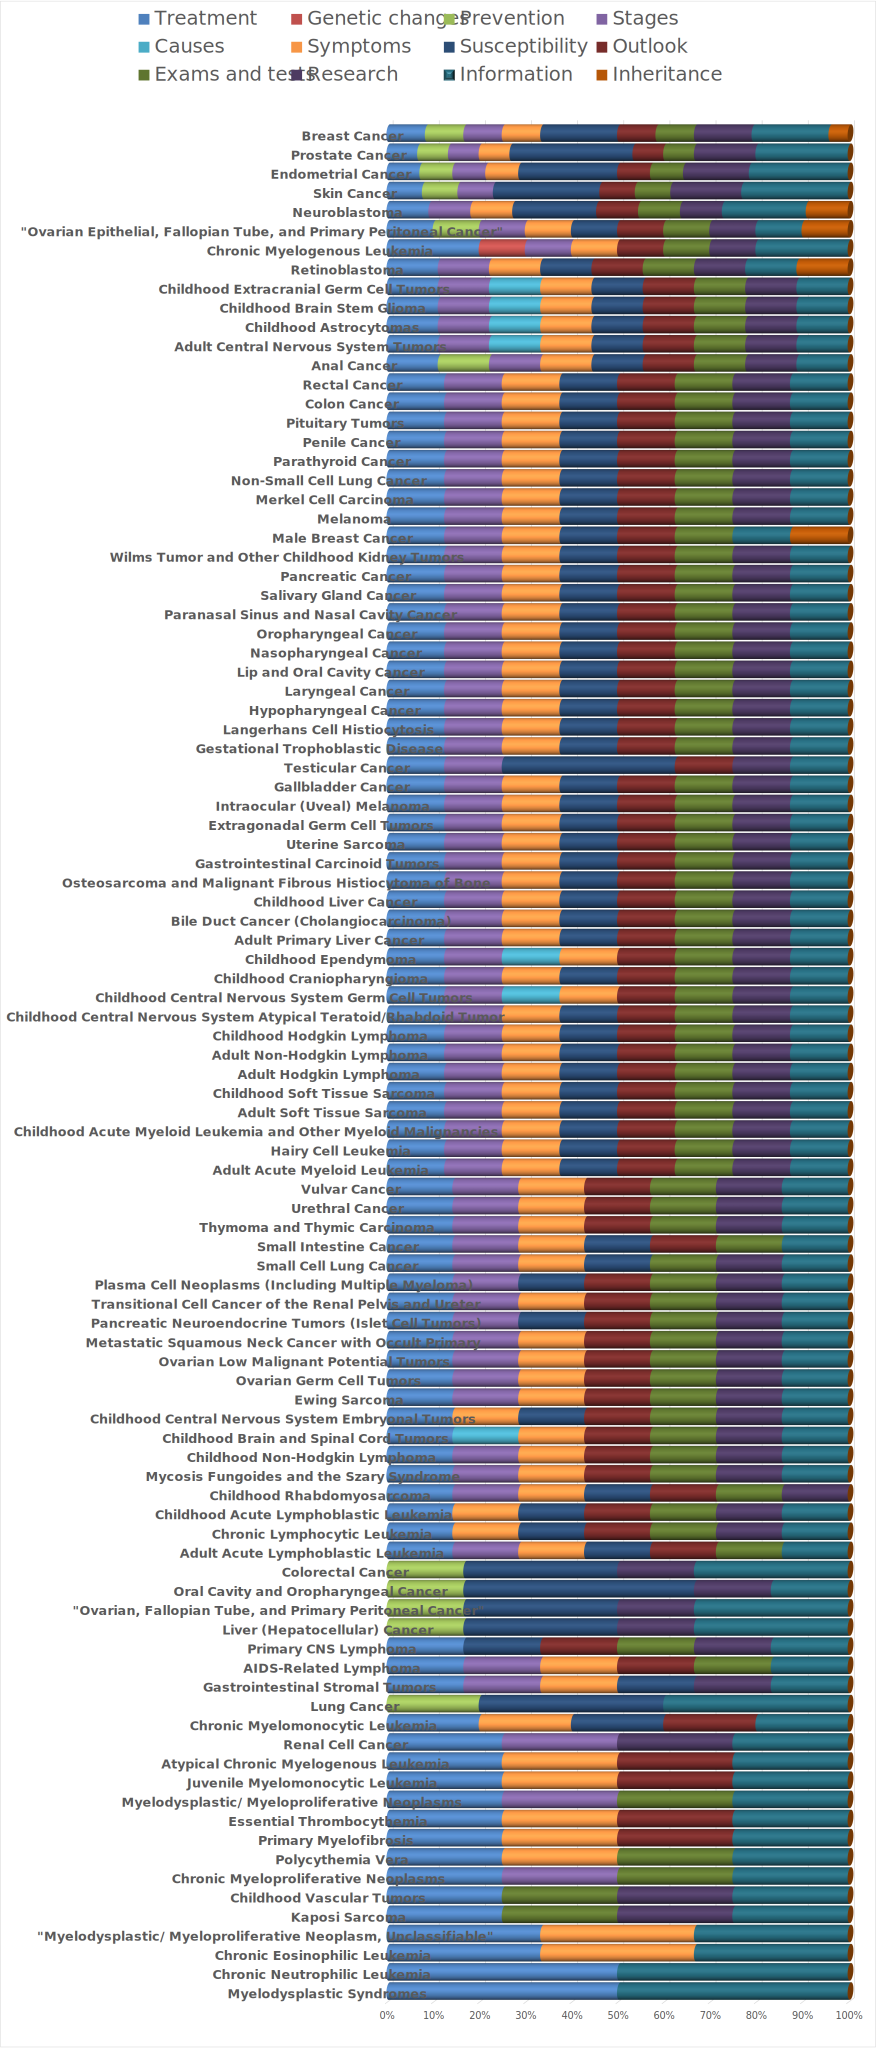
\includegraphics[scale=0.797]{Images/Cancer_qtypes.png}
	 	\caption{List of the Cancer type and question type and their count}
	 	\label{fig:cancer-type-qtype-count}
	 	\Description{A woman and a girl in white dresses sit in an open car.}
	 \end{figure}

 
 	\subsection*{Data format}
 		MedQuAD's cancer dataset are in Extensible Markup Language (XML)~\cite{MedQuAD-Cancer-dataset}, with spcific tags as shown in Table~\ref{tab:xml-tag}:
 		 	\begin{table}[ht]
 			\caption{List of the question type and their count}
 			\label{tab:xml-tag}
 			\begin{tabular}{ll}
 				\toprule
 				XML tags&Description\\
 				\midrule
 				Focus & Focus of the question\\
 				UMLS & A standardized semantic knowledge source\\
 				CUI & Concept Unique Identifier \\
 				SemanticType &  Semantic Features of questions \\
 				SemanticGroup & Semantic Group of questions\\
 				Question & The question text\\
 				Answer & The answer text\\
 				\bottomrule
 			\end{tabular}
 		\end{table}
 		
	 	For example:
	 	\begin{lstlisting}
	 		<Document id="0000001_1" source="CancerGov" url="https://www.cancer.gov/types/leukemia/patient/adult-all-treatment-pdq">
	 			<Focus>Adult Acute Lymphoblastic Leukemia</Focus>
	 			<FocusAnnotations>
 					<UMLS>
				 		<CUIs>
				 			<CUI>C0751606</CUI>
				 		</CUIs>
				 		<SemanticTypes>
				 			<SemanticType>T191</SemanticType>
				 		</SemanticTypes>
				 		<SemanticGroup>Disorders</SemanticGroup>
		 			</UMLS>
	 			</FocusAnnotations>
	 			<QAPairs>
		 			<QAPair pid="1">
			 			<Question qid="0000001_1-1" qtype="information">What is (are) Adult Acute Lymphoblastic Leukemia ?</Question>
			 			<Answer>Key Points - Adult acute lymphoblastic leukemia (ALL) is a type of cancer in which the bone marrow makes too many lymphocytes (a type of white blood cell). - Leukemia may affect red blood cells, white blood cells, and platelets. - Previous chemotherapy and exposure to radiation may increase the risk of developing ALL. - Signs and symptoms of adult ALL include fever, feeling tired, and easy bruising or bleeding. - Tests that examine the blood and bone marrow are used to detect (find) and diagnose adult ALL. ...
			 			</Answer>
	 				</QAPair>
	 			</QAPairs>
	 		</Document>
	 	\end{lstlisting}
		
		Now, by the look the data looks easy to feed into BioBERT model, however, BioBERT model requier four major components ``context'', ``question'', ``answer'', and ``start\_answer''. And the given data are missing two main parts ``context'' and ``start\_answer''. So, we have to take few manual following steps to make dataset compatible to BioBERT model.
		\begin{itemize}
			\item The give ``answer'' tags contains very big string, but the correct answer is just few lines of this text. So, we made give ``answer'' tag as ``context'' tag.
			\item Manually find the correct answer and made it as ``answer'' tag.
			\item Calculate ``start\_answer''  tag from new generated ``context'' tag
			\item finally, stored every data in JavaScript Object Notation (JSON) format.
		\end{itemize}
	
		Example of new data:
		\begin{lstlisting}
			{"data": [{
				"title": "information", 
				"paragraphs": [{
					"context": "Key Points Adult acute lymphoblastic leukemia (ALL) is a type of cancer in which the bone marrow makes too many lymphocytes (a type of white blood cell). Leukemia may affect red blood cells, white blood cells, and platelets. Previous chemotherapy and exposure to radiation may increase the risk of developing ALL. Signs and symptoms of adult ALL include fever, feeling tired, and easy bruising or bleeding. Tests that examine the blood and bone marrow are used to detect (find) and diagnose adult ALL. ...", 
					"qas": [{
						"answers": [{
							"text": "Adult acute lymphoblastic leukemia (ALL) is a type of cancer in which the bone marrow makes too many lymphocytes (a type of white blood cell).", 
							"answer_start": 11
						}], 
						"question": "What is (are) Adult Acute Lymphoblastic Leukemia ?", "id": "1"
					}]
				}],
				...}, 
				"version": "1.1", 
				"team": "nlp-group-project-fall-2020-deepbiocomp", 
				"Disease": "Cancer"
			}
		\end{lstlisting}